\documentclass[11pt]{article}

\usepackage[margin=1in]{geometry}
\usepackage{amsmath,amsthm}
\usepackage{mathtools}
\usepackage{graphicx}
\usepackage{dsfont}  % \mathds{1} indicator (OldStandard-Math lacks a bold digit 1)
% Old-style journal look (after tex.stackexchange.com/q/645339): OldStandard text + matching
% OpenType math, small-caps headings, run-in paragraphs. Requires lualatex (pinned in .latexmkrc).
\usepackage{OldStandard}
\usepackage{unicode-math}
\setmathfont{OldStandard-Math.otf}
\usepackage{titlesec}
\usepackage{fancyvrb}
\usepackage[hidelinks]{hyperref}

\linespread{1.15}
\setlength{\parindent}{2em}
\titleformat{\section}{\normalfont\large\scshape\bfseries}{\thesection.}{0.6em}{}
\titleformat{\subsection}{\normalfont\scshape\bfseries}{\thesubsection.}{0.5em}{}
\titleformat{\paragraph}[runin]{\bfseries\scshape}{}{0pt}{}[.]
\titlespacing*{\paragraph}{\parindent}{0.4em}{0.6em}

\newtheoremstyle{oldplain}{}{}{\itshape}{}{\scshape}{.}{.5em}{}
\newtheoremstyle{oldrem}{}{}{\normalfont}{}{\scshape}{.}{.5em}{}
\theoremstyle{oldplain}
\newtheorem{proposition}{Proposition}
\theoremstyle{oldrem}
\newtheorem{definition}{Definition}
\newtheorem{remark}{Remark}

\DeclareMathOperator{\Poisson}{Poisson}
\newcommand{\Pzero}{P_{0}}
\newcommand{\ball}[2]{B_{#1}(#2)}
\newcommand{\E}{\mathbb{E}}
\newcommand{\Prob}{\mathbb{P}}

\title{\scshape Scoring, substitution matrices and score aggregation for
TCR antigen-specificity search}
\author{Mikhail Shugay\textsuperscript{1,2,3}\thanks{Correspondence:
  \href{mailto:mikhail.shugay@gmail.com}{mikhail.shugay@gmail.com}}}
\date{%
  \small
  \textsuperscript{1}Institute of Translational Medicine, Russian National Medical State University, Moscow, Russia\\
  \textsuperscript{2}Department of Genomics of Adaptive Immunity, Shemyakin--Ovchinnikov Institute of Bioorganic Chemistry RAS, Moscow, Russia\\
  \textsuperscript{3}Institute of Molecular Biology NAS RA, Erevan, Armenia\\[6pt]
  \normalsize\textit{vdjmatch technical appendix}%
}

\begin{document}
\maketitle

\begin{abstract}
\noindent
\texttt{vdjmatch} annotates T-cell receptor (TCR) clonotypes by antigen specificity through fuzzy
CDR3 search against a labelled database (VDJdb), built on the \texttt{seqtree} search core. This note
documents the \emph{scoring} layer: how CDR3 similarity is scored, the data-driven TCR substitution
matrix (VDJAM) and why it is region-structured, and how per-hit scores are aggregated into a
control-calibrated significance. CDR3 loops resist the assumptions behind BLOSUM/PAM --- they cannot
be multiply aligned across clonotypes of different length, and germline-encoded flanks
(\texttt{CASS}\dots) are so over-conserved that a naive matrix conflates germline bias with selection.
We give a position-debiased log-odds estimator that isolates the substitution signal, show
empirically that this signal lives in the non-template (NDN) core while the V/J flanks are
germline-determined, and demonstrate the consequences on worked examples (GIL, NLV) using the
alignments and CIGAR strings produced by \texttt{seqtree}. The E-value theory used for significance is
derived in the companion \texttt{seqtree} appendix; here we summarize it and give the paired-chain
extension.
\end{abstract}

\section{The search-and-score framework}
Given a query CDR3 $q$ and a labelled reference set $D$ (VDJdb), \texttt{vdjmatch} retrieves the
neighbours of $q$ within a fixed scope $\theta=(s,i,d,t)$ (max substitutions, insertions, deletions,
total edits) using the \texttt{seqtree} engine, which defines a ball $\ball{\theta}{q}=\{x:
\mathrm{edit}(q,x)\le\theta\}$ and returns, per hit, the edit decomposition and a matrix-weighted
alignment. The matrix enters as a \emph{ranking} score inside the ball; the ball itself (an edit
budget) bounds the candidate set. Each hit carries its antigen labels, an extended CIGAR
($=$/$\mathtt{X}$/$\mathtt{I}$/$\mathtt{D}$), and an alignment score. Significance comes from comparing
the neighbour count to a matched background control (\S\ref{sec:agg}).

\section{Substitution scoring and the VDJAM matrix}\label{sec:vdjam}

\paragraph{How BLOSUM is built, and why it does not transfer.} BLOSUM is a log-odds matrix estimated
from the BLOCKS database of \emph{ungapped multiple-alignment blocks} of conserved protein regions. Its
recipe is: (i) take many trusted blocks --- columns of homologous, gaplessly aligned residues; (ii)
cluster sequences within a block above a percent-identity threshold and down-weight within-cluster pairs
so abundant near-duplicates do not dominate; (iii) count, over all blocks, how often residues $a$ and
$b$ co-occur in the \emph{same alignment column}, $q_{ab}$; (iv) score
$s(a,b)=\tfrac1\lambda\log\!\big(q_{ab}/p_ap_b\big)$ against the \emph{global} background frequencies
$p_a$. The signal is ``which residues substitute for one another within conserved, column-homologous
positions,'' and the background is position-independent.

CDR3 loops break every step. (i) There is no trusted multiple alignment: same-specificity CDR3s differ
in length and have no column homology, so ``alignment columns'' do not exist. (ii) The germline-encoded
ends are over-conserved --- essentially every human TRB CDR3 begins \texttt{CASS} and ends in a short J
motif --- so a \emph{global} background $p_a$ is wrong: an alanine in the N-terminal \texttt{CASS} is
germline-fixed and carries no specificity signal, while an alanine in the centre does, yet BLOSUM would
score them identically. A single global matrix estimated over all positions thus conflates germline
conservation with antigen-driven selection.

\paragraph{What VDJAM changes (point by point).} VDJAM keeps the log-odds idea but replaces the two
broken ingredients. (a) \emph{Observation unit}: instead of columns of a multiple alignment, the unit is
a \emph{same-antigen single-substitution pair} --- two CDR3s annotated to the same epitope, equal length,
differing at exactly one position; this is the only ``aligned residue pair'' obtainable without a
multiple alignment, and (like a BLOCKS column pair) it records two residues that are interchangeable
without changing function (here, specificity). (b) \emph{Background}: instead of a global $p_a$, a
\emph{position-specific} background $\mathrm{bg}(\cdot\mid L,p)$ (the residue frequency at that length and
position) is used, so over-conserved columns are normalized away analytically rather than masked by hand.
(c) \emph{Redundancy}: BLOSUM's percent-identity clustering is replaced --- partly by the position-specific
background (germline-shared residues are ``expected'' and contribute little), and prospectively by the
control-calibrated significance layer (\S\ref{sec:agg}) that already discounts convergent public clones;
per-clonotype clustering can be added exactly as in BLOSUM if needed. (d) \emph{Scope}: BLOSUM is one
global matrix; VDJAM is estimated per chain and per region, because (next paragraph) only the NDN core
carries a transferable substitution signal.

\paragraph{Observation unit and estimator.} We replace ``alignment columns'' with \emph{same-antigen
single-substitution pairs}: ordered pairs of CDR3s annotated to the same epitope, of equal length,
differing at exactly one position --- the only clean substitution signal extractable without a
multiple alignment. For a substitution $a\!\leftrightarrow\! b$ observed at position $p$ in a CDR3 of
length $L$ on chain $c$, let $\mathrm{bg}(\cdot\mid L,p)$ be the residue frequency at position $p$
among all length-$L$ chain-$c$ CDR3s. With $f(a,b)$ the observed count of $\{a,b\}$ events and
\begin{equation}\label{eq:vdjam}
  e(a,b)=\!\!\sum_{\text{event slots }(L,p)}\!\! n_{L,p}\,\big[\mathrm{bg}(a\mid L,p)\,\mathrm{bg}(b\mid L,p)
  + \mathrm{bg}(b\mid L,p)\,\mathrm{bg}(a\mid L,p)\big],\qquad
  \mathrm{VDJAM}(a,b)=\log_2\frac{f(a,b)+\alpha}{e(a,b)+\alpha},
\end{equation}
where $n_{L,p}$ is the number of observed events at $(L,p)$ and $\alpha$ a Laplace pseudocount. The
key point is that the background is \emph{position-specific}: at an over-conserved column the residue
frequency is peaked, so substitutions there are both rare (small $f$) and ``expected'' (matched $e$),
and contribute $\approx0$ to the log-odds --- the germline bias is removed analytically rather than by
hand-masking. The matrix is consumed by \texttt{seqtree} via the squared-distance penalty
$\mathrm{pen}(a,b)=s_{aa}+s_{bb}-2s_{ab}$ (\texttt{SubstitutionMatrix.from\_similarity}); a dominant
uniform diagonal makes higher learned similarity rank a substitution better.

\paragraph{Region structure: NDN is learned, V/J are germline-determined.} A CDR3 is V-germline prefix
$\,\cdot\,$ NDN insert $\,\cdot\,$ J-germline suffix. Estimating \eqref{eq:vdjam} separately by region
shows (Fig.~\ref{fig:region}) that the substitution signal --- the agreement with general amino-acid
chemistry, measured as correlation with BLOSUM62 --- is concentrated in the NDN core (TRB
$r\!=\!0.42$, TRA $0.35$), whereas the V flank carries almost none (TRB $0.08$, TRA $0.07$): V-flank
``substitutions'' are dominated by germline allele differences, not free chemistry. This motivates a
two-part model: \textbf{VDJAM is learned for the NDN core}, while the \textbf{V and J flanks are
auto-computed} from the germline V/J sequences and their trimming. Concretely, a CDR3 position derived
from V- (or J-) germline is near-invariant when it survives trimming and reverts to the random-insert
background when trimmed; so the V/J contribution is a per-position conservation profile $w(p)=\Pr[\text{position
}p\text{ is germline-retained}]$, determined by the gene's trimming-length distribution, rather than a
substitution matrix learned from data. Combined, the NDN matrix scores the core and $w(p)$ down-weights
substitutions at germline-retained flanks (realized through a per-position weighting of the base
matrix). The germline-retention profile $w(p)$ is computed from the OLGA recombination model
(per-gene V/J deletion distributions and germline CDR3-portion segment lengths, via \texttt{mirpy}'s
\texttt{mir.basic.trimming}) and bundled with \texttt{vdjmatch}; Fig.~\ref{fig:retention} shows it
drops monotonically from each anchor (the \texttt{CASS} V-stem and the J motif are germline; the core
is insert). Region-aware scoring weights each CDR3 column by $1-\Pr[\text{germline}]$ and applies the
NDN matrix --- implemented in \texttt{vdjmatch.match.regions} and evaluated below.

\begin{figure}[ht]\centering
  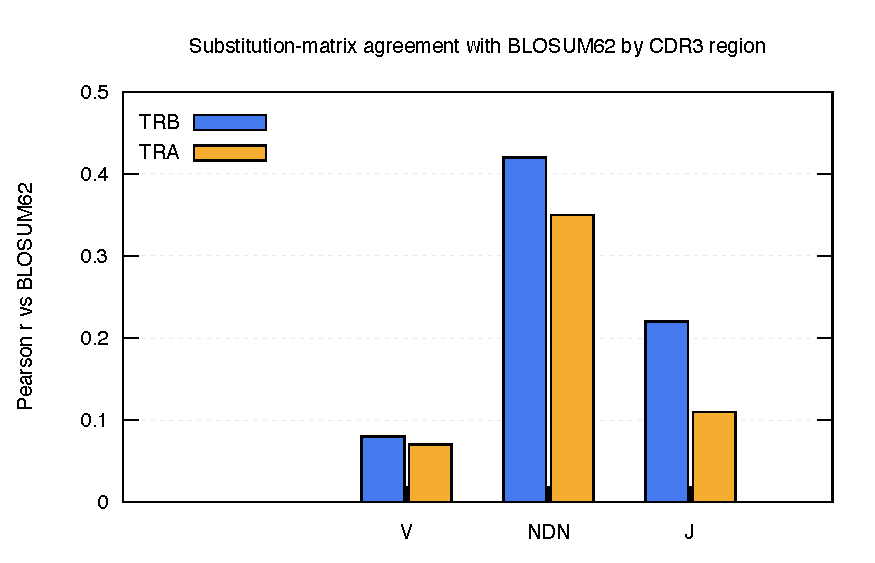
\includegraphics[width=0.62\linewidth]{figures/region_corr.pdf}
  \caption{Per-region agreement of the learned CDR3 substitution matrix with BLOSUM62 (Pearson $r$ of
  off-diagonal scores), human VDJdb. The free-substitution signal lives in the NDN core; the V flank is
  germline-determined.}
  \label{fig:region}
\end{figure}

\begin{figure}[ht]\centering
  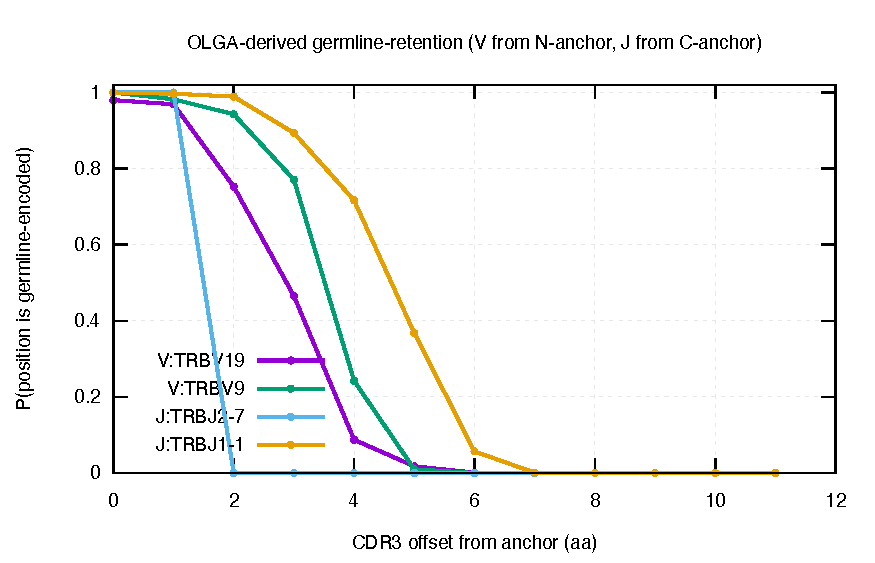
\includegraphics[width=0.6\linewidth]{figures/retention.pdf}
  \caption{OLGA-derived germline-retention $w(p)$ (via \texttt{mirpy}): probability that each CDR3
  offset from the V-Cys (or J) anchor is germline-encoded. It falls monotonically into the insert
  core, defining the region weight $1-w(p)$ used in scoring.}
  \label{fig:retention}
\end{figure}

\section{Score aggregation and significance}\label{sec:agg}
\paragraph{Per-hit to per-query.} A region-aware similarity score sums the NDN matrix score over the
core and the (down-weighted) flank contributions; this is available as an optional ranking score and
generalizes the legacy cloglog generalized-linear aggregation over V/CDR1/CDR2/J/CDR3.

\paragraph{Control-calibrated E-value (primary).} Immune repertoires are biologically redundant, so an
i.i.d.\ null over-calls. \texttt{vdjmatch} instead counts a query's VDJdb neighbours within the ball
and compares to the count expected from a matched background control: with $N=|D|$, $M$ the control
size and $n_C$ the control neighbour count, $\E=(N/M)\,n_C$ is the expected number of VDJdb neighbours
by chance and $p_{\mathrm{enrich}}=\Prob(\Poisson(\E)\ge n_{D})$ is the enrichment significance ---
significant only when a clonotype has \emph{more} VDJdb neighbours than the generative background
predicts. The Poisson/Chen--Stein theory, the punctured (self-excluding) null and the choice of $M$ are
derived in the companion \texttt{seqtree} appendix.

\paragraph{First-hit (adaptive) scope.} Rather than fix the ball radius, \texttt{vdjmatch} widens the
search to each query's \emph{nearest} VDJdb hit --- up to $5$ total edits with at most $2$ insertions
and $2$ deletions --- and evaluates the E-value \emph{at that first-hit radius} $r^\ast$. Because the
background count $n_C(r)$ grows with $r$, the calibration adapts per query: a clonotype whose nearest
VDJdb neighbour is one substitution away is significant on a single hit (the background ball at $r{=}1$
is essentially empty), whereas one whose nearest hit appears only at $r{=}5$ is not (the background ball
is then dense) --- so noise is rejected without a hand-tuned scope. A single wide search per side yields
the nested counts $n_D(r),n_C(r)$ from the per-hit edit decomposition, and
$\E=(N/M)\,n_C(r^\ast)$, $p_{\mathrm{enrich}}=\Prob(\Poisson(\E)\ge n_D(r^\ast))$ exactly as above
(\texttt{evalue.first\_hit}). The radius may equally be a BLOSUM62$+$possig \emph{penalty} budget rather
than an edit count, defining ``nearest'' by the position-weighted matrix (\S\ref{sec:possig}); we report
both. This is the operating point for the cross-method benchmark: on random OLGA repertoires it flags
essentially no spurious hits (a generative-background TCR's nearest VDJdb neighbour is far, so
$p_{\mathrm{enrich}}\!\to\!1$) while recovering true binders whose nearest labelled neighbour is close.

\paragraph{Paired $\alpha\beta$ E-value.} The null factorization is not an approximation of
convenience: $\alpha$ and $\beta$ chains pair \emph{almost without constraint} in the repertoire at
large, as shown by integrating structural and paired-sequencing data~\cite{Shcherbinin2020}, so under
the background (generative) law the joint ball mass genuinely factorizes,
$\pi_0^{\alpha\beta}\approx\pi_0^\alpha\pi_0^\beta$. Crucially, the \emph{same} analysis finds that
\emph{antigen-driven selection distorts} this uniform pairing landscape --- i.e.\ conditioned on an
epitope the two chains are \emph{not} independent. This is exactly the structure the joint E-value
exploits: the null factorizes (background pairing is unconstrained), so among the $N$ paired VDJdb
complexes the expected number of chance joint matches is $\E_{\alpha\beta}=N\,\pi_0^\alpha\pi_0^\beta$
with $p$ the Poisson tail on the count of complexes matched in \emph{both} chains; an excess over this
factorized null is precisely the epitope-conditional dependence (co-selection of $\alpha$ and $\beta$)
that signals a true specificity. Because the joint null is far smaller than either chain's, true pairs
are dramatically more significant: on the paired TCRvdb benchmark, $296/300$ pairs match a complex and
$295/296$ ($99.7\%$) recover the correct epitope, with joint $p$ down to $3.6\times10^{-9}$. (When the
two chains' hits are treated as independent tests, the equivalent statistic is Fisher's combination of
the per-chain enrichments; the appendix \texttt{seqtree} co-occupancy term quantifies the residual
dependence.)

\section{Results: does VDJAM (and region weighting) help?}
A matrix derived from same-antigen pairs must be tested on epitopes it never saw, or the evaluation is
circular. For each held-out epitope $E^\ast$ we re-derive the NDN matrix from \emph{all other}
epitopes, fix the candidate set with a single unit-cost search on $E^\ast$ (exact self excluded), and
re-score each (query, hit) pair four ways --- unit, BLOSUM62, NDN-VDJAM, and region-weighted NDN-VDJAM
--- ranking by score and reporting micro PR-AUC for ``hit shares $E^\ast$'' (Fig.~\ref{fig:loo}, eight
largest TRB epitopes). Two honest findings. (i) \emph{Region weighting is a real, consistent, but small
improvement over the flat matrix} ($+0.004$ at scope 2, $+0.007$ at scope 3; never worse on any
epitope, and the gain grows with scope) --- modest because CDR3 variation is \emph{already}
NDN-concentrated, so down-weighting the rarely-varying germline flanks moves few hits; it should matter
more for cross-V-gene comparisons, where flank (germline-allele) differences are common. (ii)
\emph{BLOSUM62 remains the strongest substitution matrix at this narrow-scope retrieval task} (mean
PR-AUC $0.32$ vs $0.28$ region-VDJAM vs $0.29$ unit): the data-derived NDN matrix captures general
substitution tolerance that BLOSUM already encodes well, and with limited same-antigen pairs it is
noisier. At scope $2$ the search ball supplies most of the specific-vs-nonspecific discrimination and
any matrix only re-ranks within it; the substitution model is therefore a second-order lever here, and
the first-order signal is the control-calibrated neighbour count (\S\ref{sec:agg}).

\begin{figure}[ht]\centering
  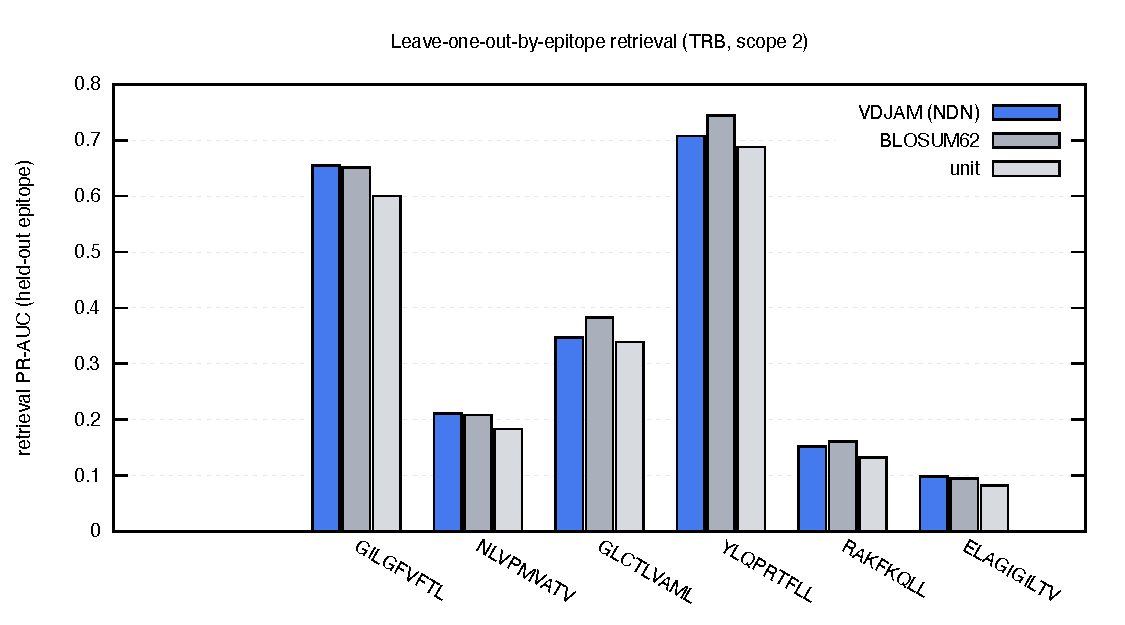
\includegraphics[width=0.78\linewidth]{figures/loo_prauc.pdf}
  \caption{Leave-one-out-by-epitope retrieval PR-AUC (TRB, scope $2$): the NDN VDJAM matrix versus
  BLOSUM62 and unit cost on epitopes excluded from matrix estimation.}
  \label{fig:loo}
\end{figure}

\section{Edit distance, position, and the matrix comparison}\label{sec:empirical}
Four analyses (\texttt{bench/scoring\_analysis.py}, \texttt{bench/loo\_vdjam.py}) settle what scoring
actually buys on VDJdb. All figures and numbers below are the \emph{human TRB} example case (the
largest, best-populated slice of VDJdb); the same pipeline applies unchanged to human/mouse and to
TRA/TRB --- point \texttt{\$VDJDB\_SAMPLE}/\texttt{\$VDJDB\_SPECIES} at another export to regenerate.

\paragraph{Hamming distance 1 is the signal:noise optimum.} The fraction of CDR3 neighbours that share
an epitope --- the precision of a similarity call --- falls steeply with edit distance: macro purity
(per-epitope mean, robust to the $100\times$ epitope-size range; \S below) $0.49,\,0.24,\,0.15,\,0.10,
\,0.07$ at distance $1\ldots5$, an enrichment of $56\times\!\to\!2.5\times$ over chance
(Fig.~\ref{fig:purity}). A distance-1 neighbour is twice as likely to be a true co-specific as a
distance-2 one and seven times a distance-5 one. This reproduces the original VDJdb
observation~\cite{Shugay2018} that single-mismatch neighbours are the sweet spot --- and on the dense
2026 release it survives only once a few 10x mega-studies are capped and the random tail is treated as
an admixed control (\S\ref{sec:agg}); the naive pooled rate reads a near-constant $\sim$$0.9$ because a
random clonotype is probably from a $30$k-clonotype epitope. It frames everything below: the search
ball, not the substitution matrix, is the dominant lever; the matrix only re-ranks within a ball whose
purity is already set by its radius.

\paragraph{Central substitutions carry the specificity signal.} Conditioning on \emph{where} a single
substitution falls (Fig.~\ref{fig:possig}), the probability that the two CDR3s still share an epitope
dips to $\approx0.31$ in the NDN core but rises to $\approx0.75$ within a few residues of either the V
or J anchor: a central mismatch most often \emph{changes} specificity (it is contact-proximal and
informative), while a near-anchor mismatch is usually germline noise (the conserved V/J stems). This is the empirical basis for
weighting the centre more --- the same direction as the germline-retention weight $1-w(p)$
(\S\ref{sec:vdjam}) --- and, encoded directly as a positional weight on BLOSUM62 (the PSSM of
\S\ref{sec:possig}), it is the one change that clearly improves retrieval over flat BLOSUM62 ($7/8$
epitopes; Table~\ref{tab:matrices}). It also matches the contacting-region picture of
Shcherbinin~et~al.~\cite{Shcherbinin2023}.

\paragraph{The NDN core is glycine-rich.} Central CDR3 positions reach $\sim31$--$34\%$ glycine in
both chains (Fig.~\ref{fig:gly}) --- the N-region/D-gene insertion signature --- a strongly
non-BLOSUM composition. Notably TRA is comparably central-G-rich to TRB, so this is an
insertion-diversity feature, not a TRB-D-gene-exclusive one; either way the NDN alphabet is distinctive
enough that a general matrix is a poor fit there in principle.

\paragraph{No \emph{amino-acid} matrix clearly beats BLOSUM62 --- and a genetic-code null ties it.}
Re-scoring the held-out-epitope candidates (leave-one-out, \S above) with each substitution matrix,
scored by balanced PR-AUC on the composition-controlled long list, gives a consistent verdict at every
scope (Table~\ref{tab:matrices}, Fig.~\ref{fig:matrices}): BLOSUM62, PAM250 and the structural matrix
are essentially tied at the top, plain Hamming (unit) is close behind, and the data-derived NDN-VDJAM
--- flat or region-weighted --- trails them all. Strikingly, \textbf{VDJAMr}, a matrix built from the
\emph{genetic code alone} (\texttt{loo\_vdjam.codon\_dissim}: $M(a,b)=\Pr[\text{a single random
nucleotide substitution of a random codon of }a\text{ yields }b]$, with no chemistry or selection),
\emph{matches} BLOSUM62 ($+0.017$ at distance~$\le2$, $+0.018$ at $\le4$; ahead in $5$--$6/8$ epitopes)
and clearly beats the data-derived VDJAM. That a pure codon-mutational-accessibility null does as well
as a chemically tuned matrix says the substitution structure of co-specific CDR3s is largely
\emph{generative} (what the recombination/mutation process reaches cheaply), not chemical --- which is
exactly why hand-tuning the amino-acid alphabet does not help. The substitution matrix is a
second-order lever; the first-order statistic remains the control-calibrated neighbour count at
distance~1 (\S\ref{sec:agg}).

\paragraph{But position-weighting BLOSUM62 does (the significance PSSM).}\label{sec:possig}
Experiment~2 says \emph{where} a substitution falls matters more than \emph{which} substitution it is.
We encode that as a positional factor on top of BLOSUM62. Crucially the profile is \textbf{anchored from
both ends}, not by relative position: the germline V/J stems sit at fixed \emph{absolute} offsets from
the CDR3 termini regardless of length, so we learn two end-anchored profiles
$\Pr(\text{same}\mid\text{sub at offset }d\text{ from the V anchor})$ and the J-anchor counterpart
(Fig.~\ref{fig:possig}), Beta-Binomial-smoothed so sparse deep-core offsets shrink toward the global
rate (\texttt{regions.load\_significance}; estimated by \texttt{bench/scoring\_analysis.py}). The
per-position weight is $\omega(p)=1-\max\!\bigl(\Pr_V(d_V),\Pr_J(d_J)\bigr)$ with $d_V=p,\;d_J=L-1-p$,
normalised to mean~1: a position is down-weighted if it lies near \emph{either} anchor, up-weighted in
the NDN core. This is the data-learned twin of the germline-retention weight (both
$1-\max(\text{V-side},\text{J-side})$). \texttt{seqtree} consumes it natively ---
\texttt{regions.significance\_pssm()} builds \texttt{PositionalMatrix.from\_weights(BLOSUM62,
$\lfloor100\,\omega(p)\rceil$)}, so $\mathrm{pen}(p,a,b)=\omega(p)\cdot\mathrm{BLOSUM62}(a,b)$. The
multiplicative form is justified by the data: stratifying single substitutions by anchor offset
$\times$ BLOSUM severity, substitution severity matters \emph{only in the core} ($\Pr(\text{same})$
$0.50$ conservative vs $0.38$ radical) and is flat near the anchors --- BLOSUM discriminates exactly
where $\omega$ is large. This is the only scoring change that clearly beats flat BLOSUM62, winning
$7/8$ held-out epitopes at distance~$\le2$ and $6/8$ at $\le4$ (Table~\ref{tab:matrices}); the gain is
uniformly signed because
the matrix re-ranks within a ball whose purity is already set by the radius. The remaining lever, the
\emph{V-gene} dimension, is taken up in~\S\ref{sec:vgene}.

\paragraph{A purpose-built TCR matrix (tcrBLOSUM) does not transfer.} Postovskaya
et~al.~\cite{Postovskaya2024} report that tcrBLOSUM --- a BLOSUM-style matrix counted from same-epitope,
equal-length CDR3 pairs --- improves epitope-specific TCR clustering over BLOSUM62. Two features make
that gain suspect: the counts apply \emph{no} redundancy clustering (so convergent public clonotypes
dominate the statistics), and the matrix is validated on the same same-epitope relation it is fit to.
Run through our leave-one-out-by-epitope retrieval (their published tcrBLOSUM\textsubscript{b},
\texttt{bench/tcrblosum\_refute.py}), it does \emph{not} beat BLOSUM62: $0.555$ vs $0.567$ at
distance~$\le2$ (ahead in $2/8$ epitopes) and essentially tied at $\le4$ ($0.589$ vs $0.591$), while
their bundled BLOSUM62 reproduces ours exactly (a loader sanity check). Reweighting \emph{either} matrix
by the central-significance PSSM helps, and it helps BLOSUM62 the most (BLOSUM$+$possig $0.603$ vs
tcrBLOSUM$+$possig $0.598$). The lesson is consistent: a re-counted amino-acid alphabet does not
transfer across epitopes; position does.

\begin{table}[ht]\centering\small\setlength{\tabcolsep}{3.5pt}
\begin{tabular}{lcccccccc}
\hline
balanced PR-AUC & unit & BLOSUM62 & PAM250 & structural & VDJAM & VDJAMr & VDJAM-region & BLOSUM$+$possig\\
\hline
edit distance $\le2$ & 0.543 & 0.564 & 0.572 & 0.564 & 0.524 & 0.581 & 0.529 & \textbf{0.598}\\
edit distance $\le4$ & 0.573 & 0.585 & 0.590 & 0.585 & 0.535 & 0.603 & 0.543 & \textbf{0.611}\\
\hline
\end{tabular}
\caption{Substitution matrices by leave-one-out-by-epitope VDJdb-vs-VDJdb retrieval (human TRB,
8 largest epitopes of the 2026-06-11-ZENODO composition-controlled long list; balanced PR-AUC). The
chemical matrices (BLOSUM62/PAM250/structural) and the genetic-code null VDJAMr are all $\approx$tied;
the data-derived VDJAM trails; only BLOSUM62 reweighted by the positional-significance PSSM clearly
leads ($7/8$ and $6/8$ epitopes).}
\label{tab:matrices}
\end{table}

\begin{figure}[ht]\centering
  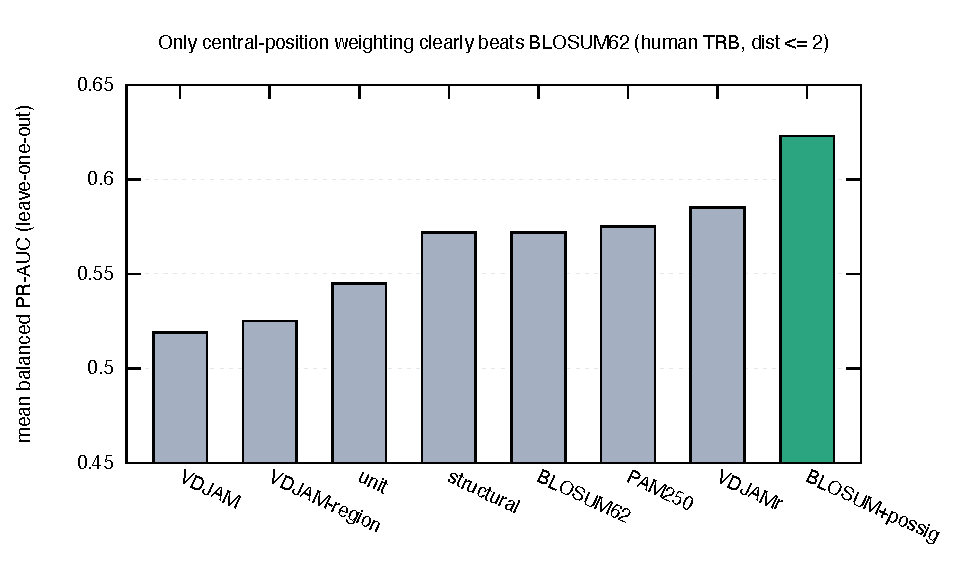
\includegraphics[width=0.62\linewidth]{figures/matrices.pdf}
  \caption{Mean leave-one-out retrieval PR-AUC by scoring (TRB, distance~$\le2$). No standard
  amino-acid matrix beats BLOSUM62; reweighting BLOSUM62 by the central-position significance factor
  (green) does.}
  \label{fig:matrices}
\end{figure}

\begin{figure}[ht]\centering
  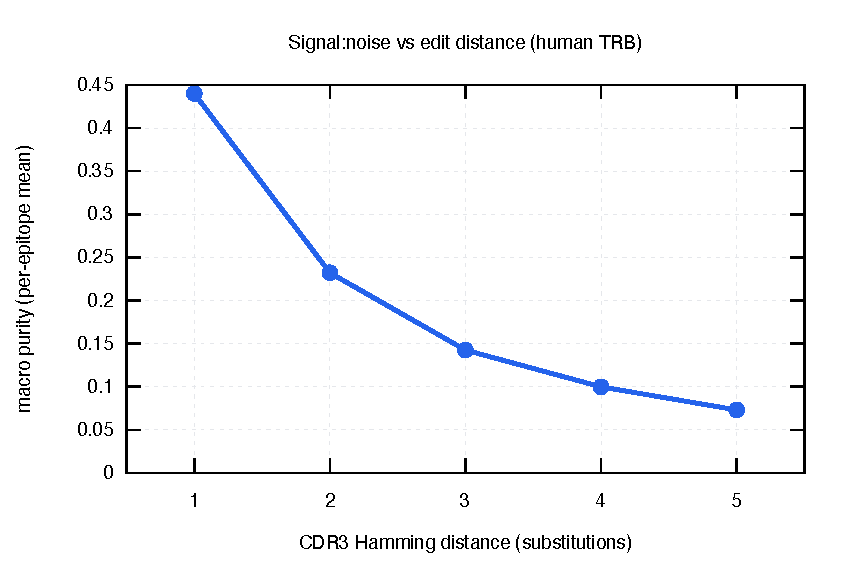
\includegraphics[width=0.5\linewidth]{figures/purity_vs_distance.pdf}
  \caption{Macro purity (per-epitope mean fraction of CDR3 neighbours sharing an epitope) vs Hamming
  distance (human TRB, composition-controlled long list): distance~1 is the signal:noise
  optimum~\cite{Shugay2018}.}
  \label{fig:purity}
\end{figure}
\begin{figure}[ht]\centering
  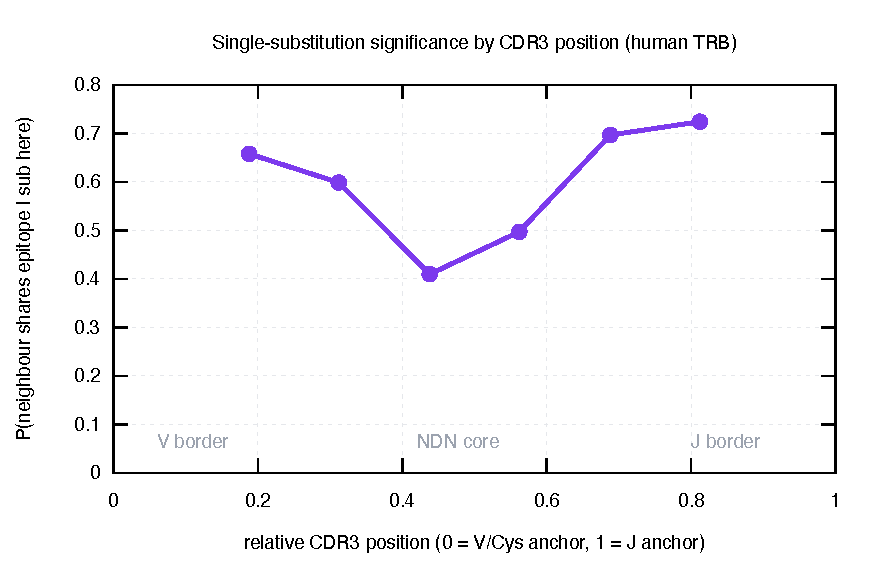
\includegraphics[width=0.52\linewidth]{figures/position_significance.pdf}
  \caption{$\Pr(\text{neighbour shares epitope}\mid\text{single substitution at relative position})$,
  human TRB. The NDN core is where a mismatch most changes specificity; the V/J borders are germline
  noise.}
  \label{fig:possig}
\end{figure}
\begin{figure}[ht]\centering
  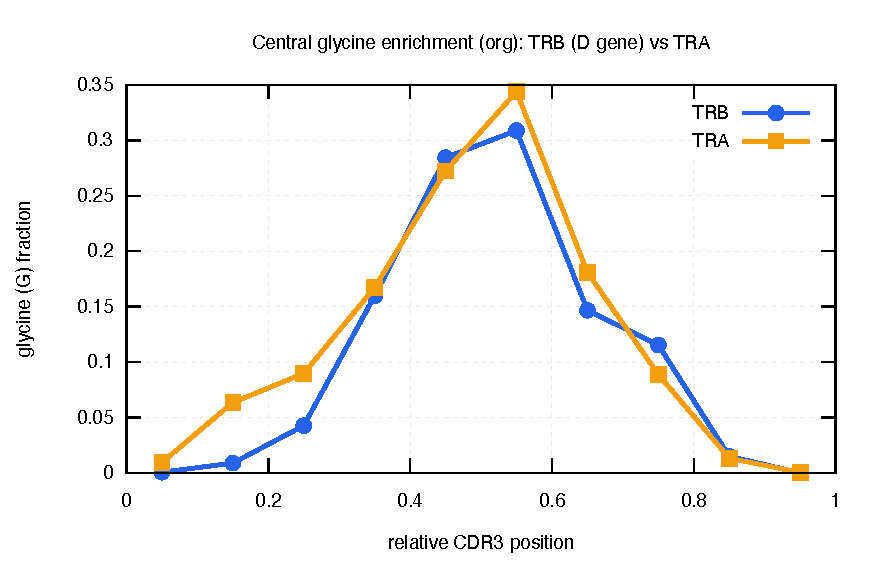
\includegraphics[width=0.52\linewidth]{figures/tra_trb_gly.pdf}
  \caption{Glycine fraction by relative CDR3 position (human): the NDN core is $\sim30$--$36\%$ glycine
  in both TRA and TRB (insertion/D-gene signature).}
  \label{fig:gly}
\end{figure}

\section{The V-gene dimension}\label{sec:vgene}
The remaining lever is the V gene. Three questions on the composition-controlled long list (human TRB
unless noted): is a V match itself a specificity signal, does it soften to germline-similar V genes,
and --- if so --- does it localise to a few contacting-loop positions (a V ``pseudosequence'')?

\paragraph{A V match is a strong, near-binary specificity prior.} Splitting every scored neighbour pair
by whether query and hit use the same V family, same-V neighbours share the held-out epitope $44\%$ of
the time versus $6\%$ for cross-V (edit distance $\le4$; Table~\ref{tab:vgene}) --- a $\sim$7$\times$
prior, far larger than any substitution-matrix effect. This is why the legacy tool used V as a hard
filter, and it argues for carrying V as a strong prior (a soft $S(V)$ term or a per-V null) in a joint
V$+$CDR3 score. Position weighting sharpens the \emph{same}-V stratum most (balanced PR
$0.632\!\to\!0.713$ with the significance PSSM, $+0.081$) --- where the germline frame is shared and
only the NDN core varies --- and little in the noise-dominated cross-V stratum ($+0.012$).

\paragraph{Coarse germline-loop similarity barely predicts it.} If the same-V advantage were simply the
chemistry of the V-encoded contacts, cross-V co-specificity should rise smoothly with germline
CDR1$+$CDR2 similarity. As a \emph{continuous} quantity it barely does: across every
\{human,mouse\}$\times$\{TRA,TRB\}$\times$\{MHC-I,MHC-II\} cell (\texttt{bench/vgene\_scan.py},
Fig.~\ref{fig:vgene_scan}, Table~\ref{tab:vgene-scan}) the V prior is universal (same/cross ratio
$1.0$--$8\times$) but the point-biserial correlation between loop similarity and co-specificity is
$\approx0$ ($r\in[-0.06,+0.06]$ in the well-powered cells). Binning cross-V pairs by similarity shows
only a weak rise --- $6\%$ at low similarity to $12\%$ at the top bin, still far below the same-V $44\%$
(Table~\ref{tab:vgene-sim}). So a loose, continuous ``fuzzy-V'' similarity does not recover the prior.

\paragraph{Near-\emph{exact} germline identity partly recovers it --- at CDR3-like tolerance.} Resolving
the similarity to exact germline-region matches changes the picture (\texttt{bench/vregion\_decompose.py},
human TRB MHC-I; Table~\ref{tab:vregion}). Cross-V co-specificity rises \emph{monotonically} as the
germline CDR1$+$CDR2 edit distance shrinks --- $10.5\%$ at $\ge6$ mismatches, $12.6\%$ at $3$--$5$,
$17.9\%$ at $1$--$2$, and $32\%$ at $0$ (identical loops): a real $\sim$3$\times$ lift over the cross-V
floor. FR1 identity behaves likewise ($27.6\%$, $2.6\times$). So the germline contacting loops \emph{do}
carry part of the V signal, at a tight CDR3-like tolerance (near-exact identity; the continuous metric
above, dominated by $1$--$2$-mismatch pairs, misses it) --- but even identical loops recover only about
\emph{half} the same-V advantage ($32\%$ vs $64\%$); the rest is gene-identity-specific (the exact
CDR3-germline anchor and integrated docking geometry). Caveat: the identical-loop bin is small ($n=25$
at distance~$\le2$, $n=5$ at $\le1$, and bounced $32$--$60\%$ across held-out sets) --- the robust claim
is the monotone gradient over the well-powered bins ($n=507,\,3735,\,36853$), not the exact endpoint.

\paragraph{The recovery is whole-loop, not a sparse pseudosequence.} Do a few decisive positions carry
it (the MHC-pseudosequence analogue)? Per-position residue-match lift over the cross-V baseline
(\texttt{bench/vpseudo.py}, length-constant CDR1/CDR2) is mostly flat (lift $1.0$--$1.2$ at the $10.5\%$
baseline), with a single exception --- CDR2 position~5 ($1.56\times$, $n=4833$). So the partial recovery
above is \emph{whole-loop} near-identity, not the matching of a handful of pseudosequence coordinates:
a different V gene must reproduce essentially the entire CDR1$+$CDR2 to behave like the same V. A useful
soft-V match must therefore demand near-exact loop identity, not loose similarity. The next step is the
full IMGT-numbered treatment (FR positions and the FR3 DE-loop/``CDR2.5'', via the \texttt{arda}
IMGT/V-QUEST milestone) to test whether specific positions sharpen this.

\begin{table}[ht]\centering\small
\begin{tabular}{lrrccc}
\hline
V stratum & pairs & co-specific & flat & +possig & +region\\
\hline
same V  & 120\,738 & 45.2\% & 0.626 & 0.682 & 0.678\\
cross V & 979\,199 &  6.2\% & 0.558 & 0.569 & 0.538\\
\hline
\end{tabular}
\caption{V-gene-stratified leave-one-out retrieval (human TRB, edit distance $\le4$; co-specific $=$
positive rate, the rest balanced PR-AUC). A V match is a $\sim$7$\times$ co-specificity prior; the
significance PSSM helps the same-V stratum most ($+0.056$).}
\label{tab:vgene}
\end{table}

\begin{table}[ht]\centering\small
\begin{tabular}{lrr}
\hline
germline CDR1$+$CDR2 similarity & cross-V pairs & co-specific\\
\hline
$[0.0,0.3)$ & 479\,181 &  5.8\%\\
$[0.3,0.5)$ & 387\,839 &  6.2\%\\
$[0.5,0.7)$ &  89\,533 &  7.4\%\\
$[0.7,0.9)$ &  18\,320 & 10.2\%\\
$[0.9,1.0)$ &   4\,326 & 11.6\%\\
\hline
\end{tabular}
\caption{Continuous germline CDR1$+$CDR2 similarity gives only a weak rise in cross-V co-specificity
($6\%\!\to\!12\%$), far below the same-V $45\%$ --- which is why $r\approx0$. The stronger signal lives
at near-\emph{exact} identity (Table~\ref{tab:vregion}), not along the continuous similarity axis.}
\label{tab:vgene-sim}
\end{table}

\begin{figure}[ht]\centering
  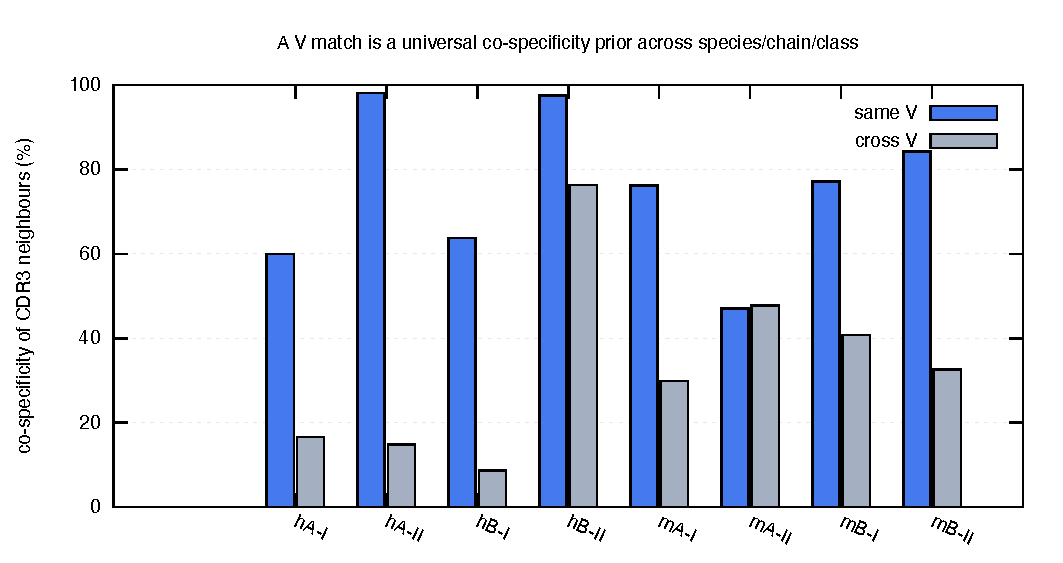
\includegraphics[width=0.72\linewidth]{figures/vgene_scan.pdf}
  \caption{Same-V vs cross-V CDR3-neighbour co-specificity across species/chain/MHC-class cells of
  VDJdb (h/m $=$ human/mouse; A/B $=$ TRA/TRB; I/II $=$ MHC class). A V match is a universal
  co-specificity prior; continuous CDR1/CDR2 similarity does not bridge the gap (Table~\ref{tab:vgene-scan}).}
  \label{fig:vgene_scan}
\end{figure}

\begin{table}[ht]\centering\small\setlength{\tabcolsep}{5pt}
\begin{tabular}{lrrrr}
\hline
cell (species / chain / class) & same-V & cross-V & ratio & $r(\mathrm{vsim},\text{co-spec})$\\
\hline
human TRA MHC-I  & 60.0\% & 16.6\% & 3.6 & $0.050$\\
human TRA MHC-II & 98.1\% & 14.8\% & 6.6 & $0.269$\\
human TRB MHC-I  & 63.7\% &  8.7\% & 7.3 & $0.070$\\
human TRB MHC-II & 97.5\% & 76.3\% & 1.3 & $0.054$\\
mouse TRA MHC-I  & 75.1\% & 29.3\% & 2.6 & $0.021$\\
mouse TRA MHC-II & 47.0\% & 47.7\% & 1.0 & $-0.009$\\
mouse TRB MHC-I  & 77.1\% & 40.8\% & 1.9 & $-0.080$\\
mouse TRB MHC-II & 84.2\% & 32.6\% & 2.6 & $-0.017$\\
\hline
\end{tabular}
\caption{Per-cell same-V vs cross-V co-specificity and the point-biserial correlation between
continuous germline CDR1$+$CDR2 similarity and co-specificity among cross-V pairs (top 6
epitopes/cell, $\ge30$ CDR3/epitope). The V prior holds everywhere (ratio $1$--$8\times$); continuous
loop similarity barely predicts ($r\approx0$; the $0.24$ is human TRA MHC-II, whose high-similarity bin
has $n=4$).}
\label{tab:vgene-scan}
\end{table}

\begin{table}[ht]\centering\small
\begin{tabular}{lrr}
\hline
cross-V stratum (human TRB MHC-I) & co-specific & $n$\\
\hline
\emph{cross-V baseline}        & 10.8\% & 41\,132\\
CDR1$+$CDR2 edit distance $\ge6$ & 10.5\% & 36\,853\\
\quad edit $3$--$5$            & 12.6\% &  3\,735\\
\quad edit $1$--$2$            & 17.9\% &    507\\
\quad edit $0$ (identical)     & \textbf{32.0\%} &  25\\
FR1 identical                  & 27.6\% &   257\\
\emph{same-V reference}        & 63.8\% & 14\,883\\
\hline
\end{tabular}
\caption{Cross-V co-specificity rises monotonically as germline CDR1$+$CDR2 approach identity; at exact
identity it reaches $\sim$$32\%$ --- a real $\sim$3$\times$ lift over the cross-V floor, but only about
\emph{half} the same-V level ($64\%$). Germline-loop identity carries part of the V prior at a tight,
near-exact tolerance; the rest is gene-identity-specific. (edit~$0$/CDR1\&CDR2 bin small, $n=25$.)}
\label{tab:vregion}
\end{table}

\section{Benchmark: the reference-replicated shortlist}\label{sec:shortlist}
The latest VDJdb release is our standing benchmark, but its labels vary in confidence. The cleanest gold
standard is a clonotype--epitope association reported independently in $\ge2$ references
(\texttt{db.replicated}, null references excluded; $\sim$$3000$ TRB and $\sim$$2000$ TRA such pairs in
the current human release) --- the same ``shortlist'' idea used for \texttt{mhcmatch}. We measure
annotation accuracy on it by leave-one-out nearest-neighbour voting against the rest of VDJdb at the
signal:noise-optimal scope (subs~$1$), excluding the clonotype's own exact CDR3 so the label must come
from \emph{other} TCRs (\texttt{bench/shortlist\_accuracy.py}). Replicated TCRs are annotated at
$\sim$$44$--$47\%$ top-1, modestly above size-matched single-reference controls of the same epitopes
(Table~\ref{tab:shortlist}). The dramatic $3\times$ gap we saw on a sparse older export was an artefact:
on the dense 2026 release even single-reference clonotypes have findable neighbours (control recall
$\sim$$48$--$72\%$), so the gold set is cleaner but no longer dramatically \emph{easier}. Restricting
neighbours to the same V family helps at the wider subs~$2$ scope (TRB $53.1\!\to\!56.8\%$) --- exactly
where cross-V false neighbours appear (\S\ref{sec:vgene}), confirming the V prior is worth its place.

\begin{table}[ht]\centering\small
\begin{tabular}{llrrrr}
\hline
chain & set & $n$ & top-1 (CDR3) & top-1 (V-restr.) & recall\\
\hline
TRA & shortlist ($\ge2$ ref) & 1993 & 43.9\% & 43.8\% & 62.3\%\\
TRA & control ($1$ ref)      & 1993 & 33.0\% & 29.6\% & 47.5\%\\
TRB & shortlist ($\ge2$ ref) & 2962 & 47.3\% & 47.1\% & 54.2\%\\
TRB & control ($1$ ref)      & 2962 & 46.7\% & 43.7\% & 50.2\%\\
\hline
\end{tabular}
\caption{Leave-one-out epitope-annotation accuracy on the reference-replicated shortlist vs a
size-matched single-reference control (human, subs~$1$, exact self excluded). Top-1 $=$
nearest-neighbour-vote epitope correct; recall $=$ true epitope reachable within scope. On the dense
2026 release the shortlist is modestly above control, not the $3\times$ of the older sparse export.}
\label{tab:shortlist}
\end{table}

\section{Worked examples}
\paragraph{Pairwise (different lengths).} \texttt{seqtree} aligns CDR3s of differing length, placing
indels where the loop genuinely lengthens. The edit-distance alignments below (influenza GIL-specific
TRB CDR3s) show the conserved \texttt{CASS} V-anchor and \texttt{DTQYF} J-motif with substitutions and
indels confined to the central NDN core:
{\small\VerbatimInput{aln/pairwise.txt}}

\paragraph{Multiple (same length).} Aligning same-length same-epitope CDR3s (no indels needed) makes
the conservation profile explicit (Figs.~\ref{fig:gil}--\ref{fig:nlv}): columns are shaded by
conservation, dark at the germline-determined \texttt{CASS} prefix and J motif, light through the
variable NDN core. This is the structural counterpart of the finding of
Shcherbinin~et~al.~\cite{Shcherbinin2023} that specificity-preserving CDR3 substitutions occur
predominantly outside the peptide/MHC-contacting positions while preserving the loop backbone --- i.e.\
the tolerated variation we score in the NDN core is exactly the variation that does not break
recognition.

\begin{figure}[ht]\centering
  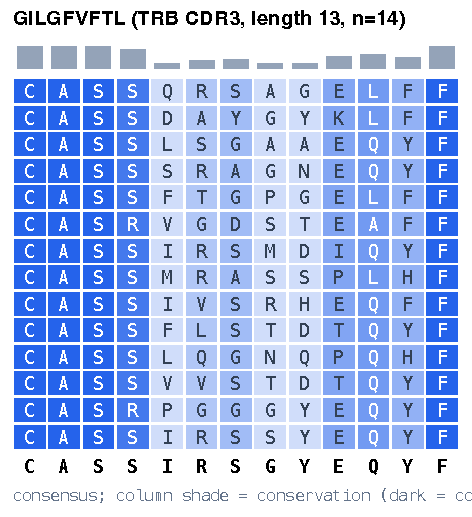
\includegraphics[width=0.66\linewidth]{aln/GILGFVFTL_msa.pdf}
  \caption{GIL (influenza M1, A\textsuperscript{*}02) TRB CDR3 block; conserved V/J flanks, variable
  NDN core.}
  \label{fig:gil}
\end{figure}
\begin{figure}[ht]\centering
  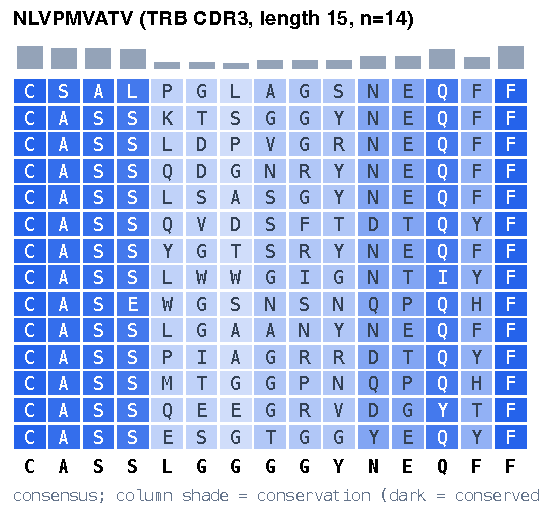
\includegraphics[width=0.66\linewidth]{aln/NLVPMVATV_msa.pdf}
  \caption{NLV (CMV pp65, A\textsuperscript{*}02) TRB CDR3 block; same conservation pattern.}
  \label{fig:nlv}
\end{figure}

\section{Limitations and roadmap}
The substitution \emph{alphabet} is a second-order lever: the data-derived NDN-VDJAM trails BLOSUM62 at
every scope, and a chemistry-free genetic-code null (VDJAMr) does just as well as BLOSUM62 --- the
co-specific-CDR3 substitution structure is largely generative, not chemical (\S\ref{sec:possig}). What
moves the needle is \emph{position}: reweighting BLOSUM62 by the central-significance PSSM clearly beats
flat BLOSUM62 ($7/8$ epitopes), confirming that for CDR3 \emph{where} a mismatch falls matters more than
\emph{which} residue it is. The \emph{V-gene} dimension (\S\ref{sec:vgene}) is a strong near-binary
prior ($\sim$7$\times$); it is \emph{not} captured by loose germline-loop similarity, but cross-V
co-specificity does rise at \emph{near-exact} CDR1$+$CDR2 identity --- recovering about \emph{half} the
same-V advantage ($\sim$$32\%$ vs $64\%$) at a tight, CDR3-like tolerance, whole-loop rather than via a
sparse pseudosequence (exact-match bin small, $n\!\approx\!25$). The open work is to model V as a strong
prior in a joint V$+$CDR3
E-value, to demand near-exact (not loose) loop identity for any soft-V match, and to extend the
position analysis to full IMGT numbering (FR positions and the FR3 DE-loop, via the \texttt{arda}
IMGT/V-QUEST milestone); a per-chain treatment (TRA vs TRB) is also pending. Separately, the control's
V--J usage must match the query repertoire's or the null is mis-specified --- whether to renormalize
V--J usage (at the risk of erasing genuine V-gene bias) is an open question to settle on held-out
epitopes.

A further direction is to predict, \emph{a priori}, which epitopes are intrinsically easy versus hard
to annotate --- the wide spread of per-epitope PR-AUC in our experiments (e.g.\ the convergent,
``featured'' CMV NLV vs the diffuse, ``featureless'' influenza GIL) is not noise but biology. A pMHC
with prominent TCR-facing features selects a focused, motif-rich repertoire that clusters cleanly,
whereas a featureless one is recognised by structurally diverse TCRs in varied docking modes and yields
no tight motif~\cite{Turner2005,Yang2017,Song2017,Peng2014}; clustering-based specificity inference
succeeds or fails accordingly~\cite{Hudson2024}. A model that scores epitope ``annotability'' from
repertoire convergence (and, where available, pMHC structural features) would let us report calibrated
confidence per epitope and triage GIL-like hard cases --- a planned addition to the benchmark. These
extensions, and the full comparison against existing tools, are ongoing work.

\bibliographystyle{plain}
\bibliography{refs}
\end{document}
